% do not change these two lines (this is a hard requirement
% there is one exception: you might replace oneside by twoside in case you deliver 
% the printed version in the accordant format
\documentclass[11pt,titlepage,oneside,openany]{article}
\usepackage{times}
\usepackage{tcolorbox}
\usepackage{enumitem}

\usepackage{subcaption} 
\usepackage{graphicx}
\usepackage{latexsym}
\usepackage{amsmath}
\usepackage{amssymb}
\usepackage{multicol}
\usepackage{hyperref}

\usepackage{ntheorem}

% \usepackage{paralist}
\usepackage{tabularx}

% this packaes are useful for nice algorithms
\usepackage{algorithm}
\usepackage{algorithmic}

% well, when your work is concerned with definitions, proposition and so on, we suggest this
% feel free to add Corrolary, Theorem or whatever you need
\newtheorem{definition}{Definition}
\newtheorem{proposition}{Proposition}


% its always useful to have some shortcuts (some are specific for algorithms
% if you do not like your formating you can change it here (instead of scanning through the whole text)
\renewcommand{\algorithmiccomment}[1]{\ensuremath{\rhd} \textit{#1}}
\def\MYCALL#1#2{{\small\textsc{#1}}(\textup{#2})}
\def\MYSET#1{\scshape{#1}}
\def\MYAND{\textbf{ and }}
\def\MYOR{\textbf{ or }}
\def\MYNOT{\textbf{ not }}
\def\MYTHROW{\textbf{ throw }}
\def\MYBREAK{\textbf{break }}
\def\MYEXCEPT#1{\scshape{#1}}
\def\MYTO{\textbf{ to }}
\def\MYNIL{\textsc{Nil}}
\def\MYUNKNOWN{ unknown }
% simple stuff (not all of this is used in this examples thesis
\def\INT{{\mathcal I}} % interpretation
\def\ONT{{\mathcal O}} % ontology
\def\SEM{{\mathcal S}} % alignment semantic
\def\ALI{{\mathcal A}} % alignment
\def\USE{{\mathcal U}} % set of unsatisfiable entities
\def\CON{{\mathcal C}} % conflict set
\def\DIA{\Delta} % diagnosis
% mups and mips
\def\MUP{{\mathcal M}} % ontology
\def\MIP{{\mathcal M}} % ontology
% distributed and local entities
\newcommand{\cc}[2]{\mathit{#1}\hspace{-1pt} \# \hspace{-1pt} \mathit{#2}}
\newcommand{\cx}[1]{\mathit{#1}}
% complex stuff
\def\MER#1#2#3#4{#1 \cup_{#3}^{#2} #4} % merged ontology
\def\MUPALL#1#2#3#4#5{\textit{MUPS}_{#1}\left(#2, #3, #4, #5\right)} % the set of all mups for some concept
\def\MIPALL#1#2{\textit{MIPS}_{#1}\left(#2\right)} % the set of all mips

% Requirements
% Main findings
% Things we tried and did not work
% max 10 pages




\begin{document}

\pagenumbering{roman}
% lets go for the title page, something like this should be okay
\begin{titlepage}
	\vspace*{2cm}
  \begin{center}
    {\Large Use of Framing Concepts to explain Discrimination in Newspapers\\}
   % \textbf{Data Dream Team \\}
    \vspace{2cm} 
   {Computational Analysis of Communication Report\\}
   \vspace{1.5cm}
   {presented by\\
   Robin-Kiara Braun (1694244)\\
   Marmee Pandya (1963521) \\
   }
   \vspace{1cm} 
   {submitted to \\
    Prof.\ Rainer Freudenthaler\\
    University of Mannheim\\} \vspace{2cm}
   {24th June 2026}
  \end{center}
\end{titlepage} 

\bibliographystyle{plain}

% no lets make some add some table of contents
% \tableofcontents
% \newpage

% \listofalgorithms

% \listoffigures

% \listoftables

% evntuelly you might add something like this
% \listtheorems{definition}
% \listtheorems{proposition}

% \newpage


% okay, start new numbering ... here is where it really starts




\pagenumbering{arabic}

\section{Project outline}
\label{cha:businessUnderstanding}

- 12 pages max. per person 
- What we improved and annotated to get better results 


\section{Annotation Instructions}
\label{cha:Instructions LLM}
\begin{itemize}
    \item Looking at security threat and benefit framing
    \item Theories to use: 
    \begin{itemize}
        \item Immigration and Racial Minority Framing
        \item Framing Theory
    \end{itemize}
\end{itemize}

Haben Annotation instruction so gewählt nach Codebook dass Kriege nicht mit rein zählen da wir uns ja anschauen möchten wie die berichterstattung ausserhalb von kriegen ist bei denen die Nationalität ja aus jornalistischen gründen/ aufklärung genannt wird. 
Nicht um Immigrants in ein schlechtes Bild au rücken. 

\begin{itemize} 
\item Input Paper \textit{Do News Frames Really Have Some Influence in the Real World? A Computational Analysis of Cumulative Framing Effects on Emotions and Opinions About Immigration}
    \begin{itemize}
        \item a news frame refers to “the central organizing idea for news content that supplies a context and suggests what the issue is” (Tankard et al. 1991: 3).
        \item A framing effect occurs when the media message interacts with prior knowledge to affect an individual’s understanding, opinion, emotion, or behavior toward an object (Lecheler and De Vreese 2019). 
        \item the crime frame describes immigration and immigrants as threats to a nation’s safety
        \item Lahav and Courtemanche’s (2012) experiment revealed that the crime frame tends to have a stronger impact than the culture frame in influencing the audience’s policy preference and that liberal-leaning participants were more responsive to the framing effect than conservatives.
        \item Igartua et al. (2011) found that the crime frame produced a significant effect on the participants’ emotions.
    \end{itemize}
\end{itemize}

\begin{itemize} 
\item Input Paper \textit{(In)direct Framing Effects: The Effects of News Media Framing on Public Support for Turkish Membership in the European Union}
 \begin{figure}[htbp]
    \centering
    \begin{subfigure}{0.48\textwidth}
        \centering
        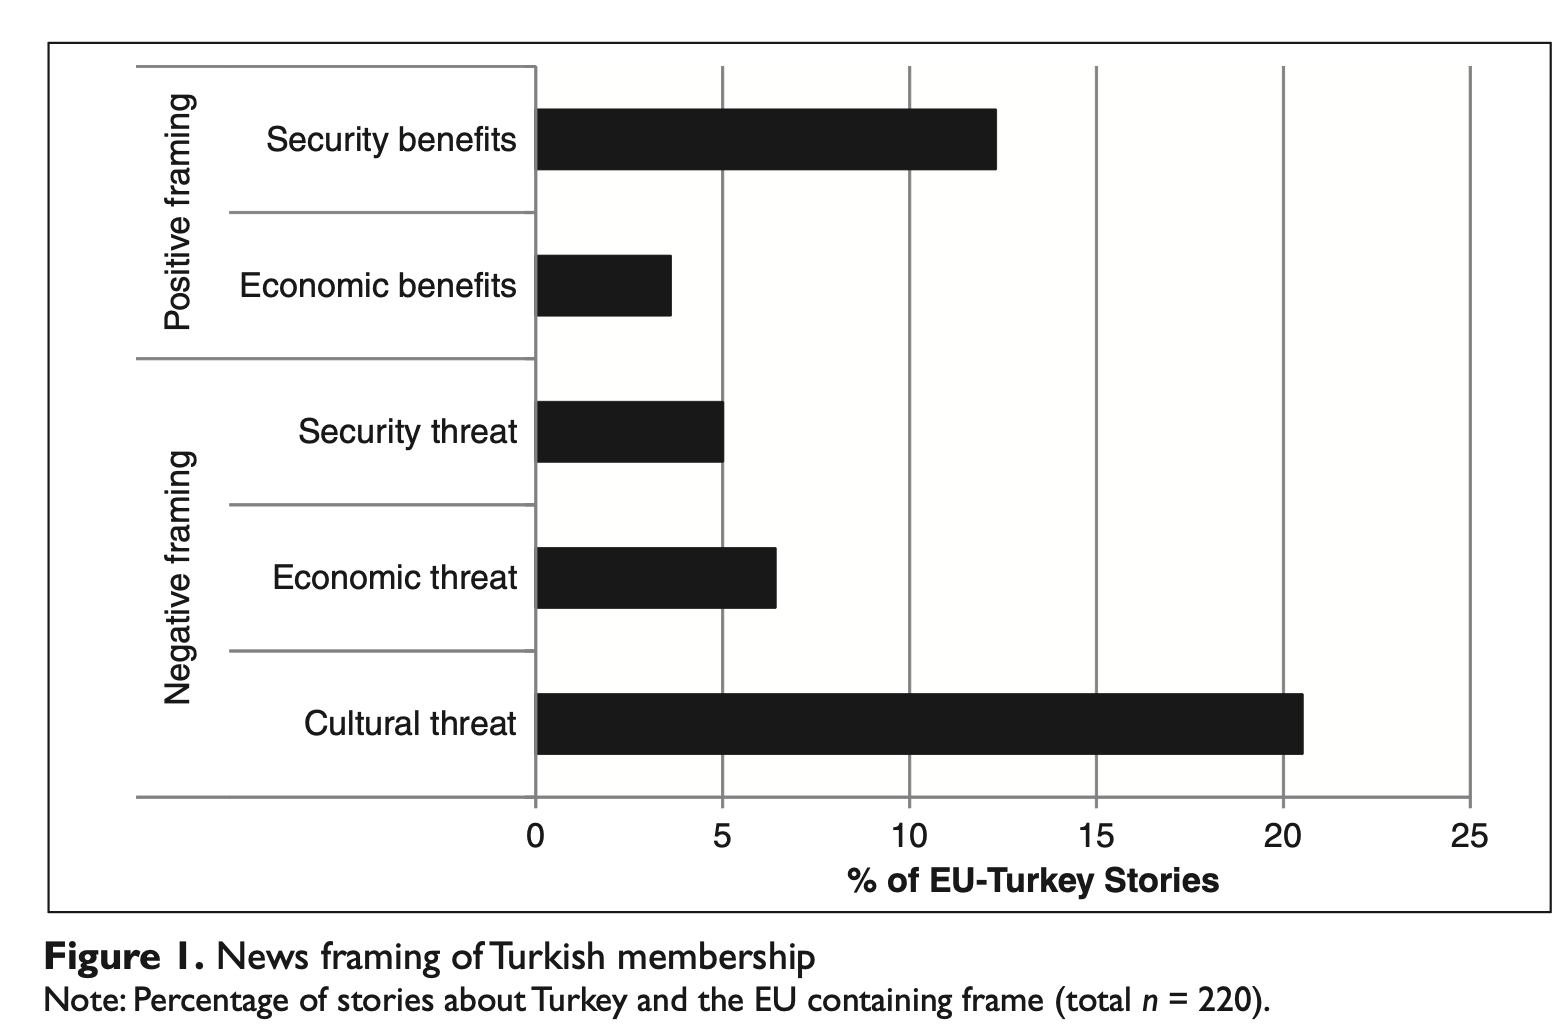
\includegraphics[width=\linewidth]{News Framing of Turkish membership.png}
        \caption{News framing of Turkish membership}
        \label{fig:news_framing_turkish_membership}
    \end{subfigure}
    \hfill
    \begin{subfigure}{0.48\textwidth}
        \centering
        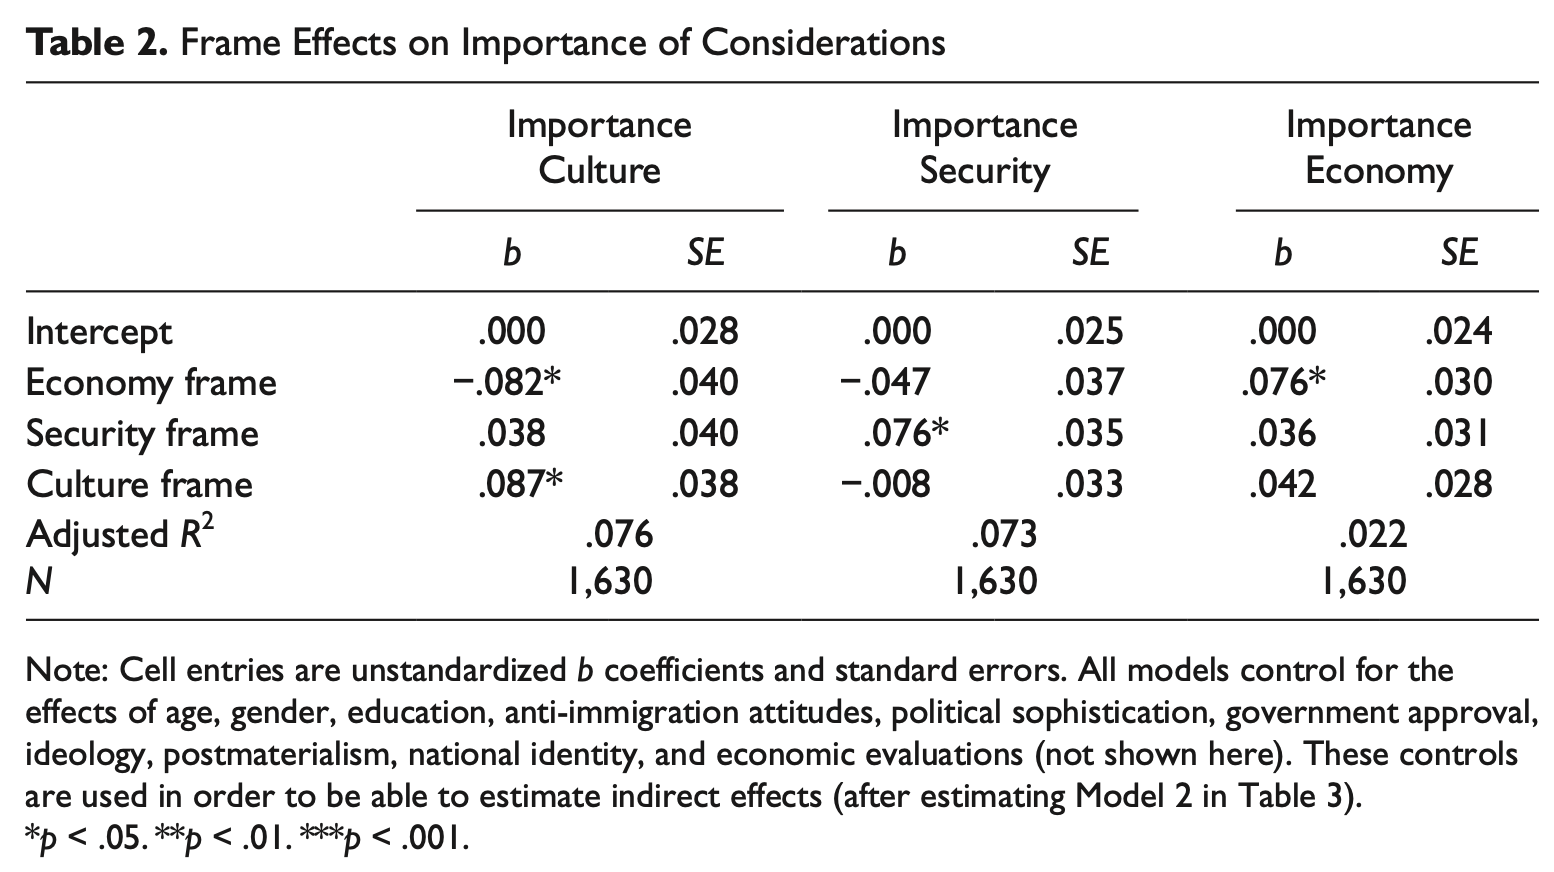
\includegraphics[width=\linewidth]{Frame Effects.png}
        \caption{Frame Effects}
        \label{fig:frame_effects}
    \end{subfigure}
    \caption{Comparison of news framing and frame effects}
    \label{fig:combined_frames}
\end{figure} 

    \begin{itemize}
        \item Five percent of all EU Turkey news stories used a security threat frame. These findings show that frames are positively and negatively valenced and that negative frames were relatively more prominent than positive frames.
    \end{itemize}
\begin{figure}
    \centering
    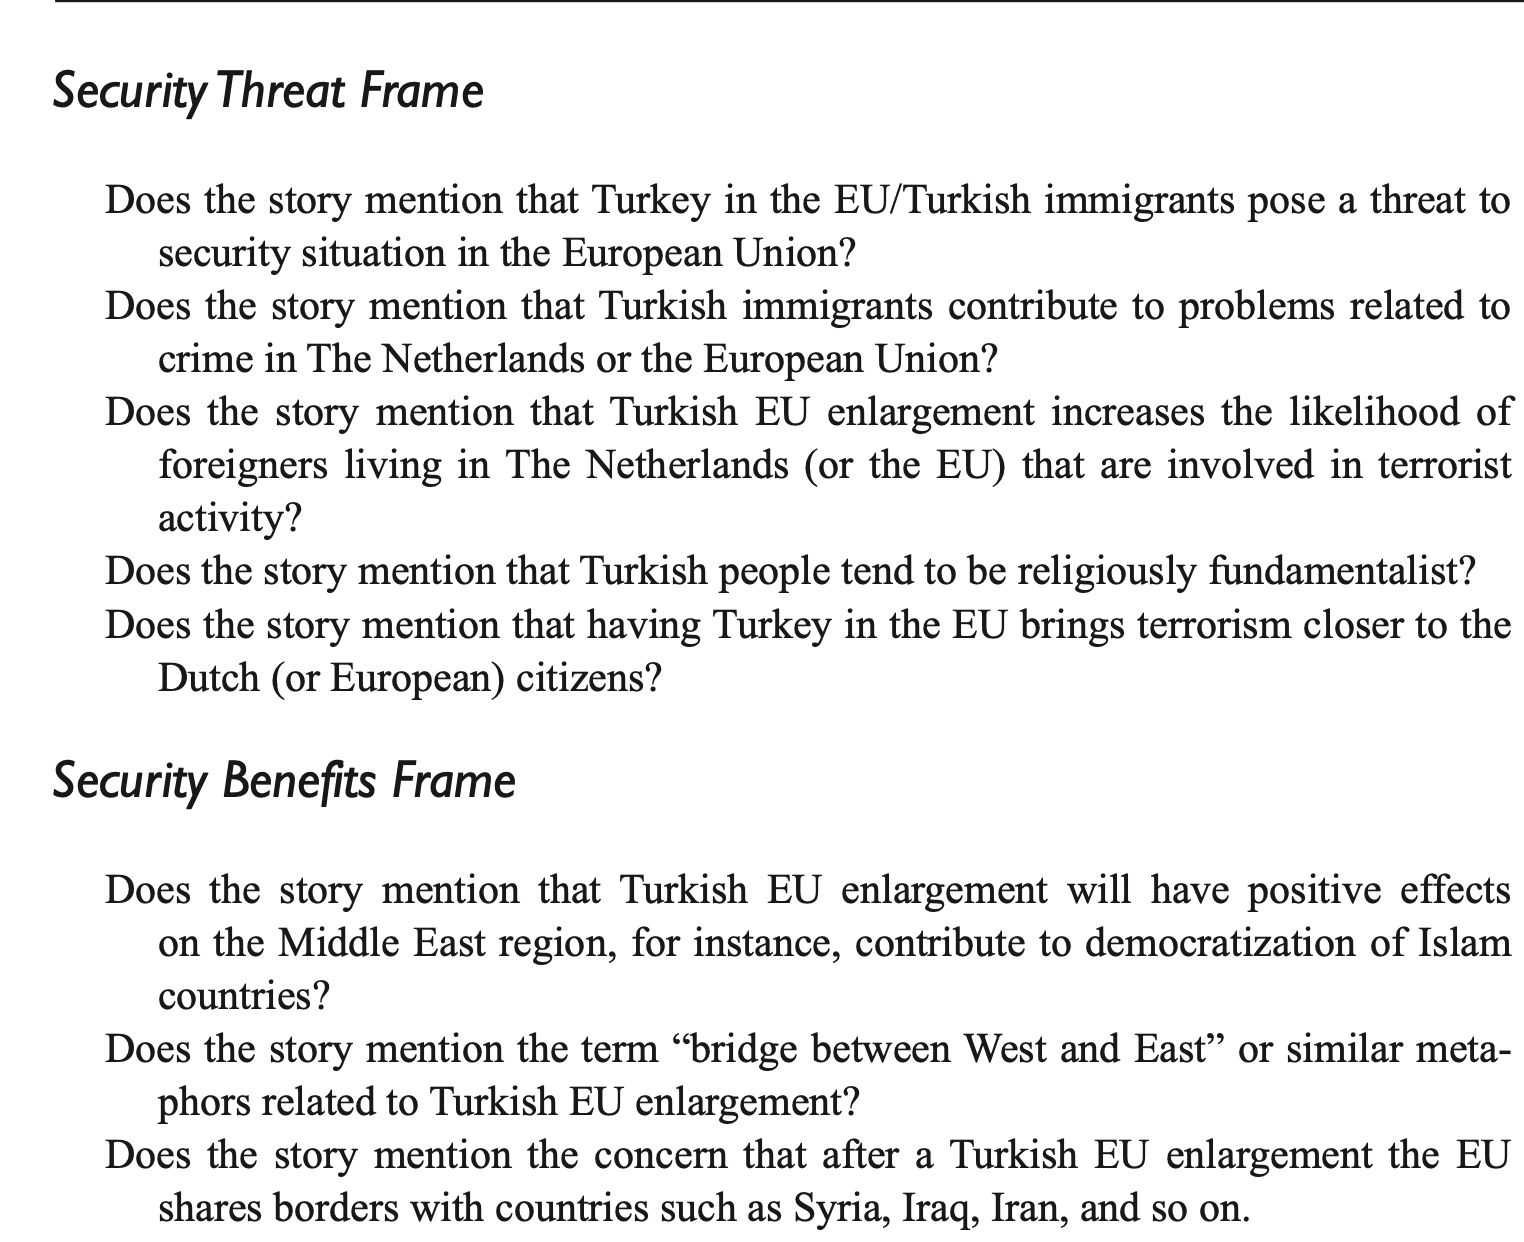
\includegraphics[width=0.75\linewidth]{FramingQuestions.png}
    \caption{Framing Questions}
    \label{fig:placeholder}
\end{figure}

\newtcolorbox{instructionbox}{
  colback=white,
  colframe=black,
  boxrule=0.8pt,
  arc=0pt,
  breakable,
  enhanced
}
\begin{instructionbox}

\textbf{Annotation Instructions:}
\textbf{Role description}

You are a neutral annotation assistant. Your task is to classify whether a single data row contains an explicit security or crime frame and, if so, whether that frame is presented positively or negatively. Annotate one row at a time and judge only the text provided in that row.

\medskip
\textbf{Context}

The data come from German newspaper articles published in 2022. Outlets include national newspapers, regional newspapers, and alternative media. Available fields may include \texttt{article\_id}, \texttt{pub}, \texttt{par\_index}, \texttt{text\_block}, \texttt{group}, \texttt{length}, and \texttt{text\_block\_en}.

Use \texttt{text\_block} as the main evidence because it is the original German text. Use \texttt{text\_block\_en} only as a backup if needed for comprehension. Group identities are anonymized and may appear as \texttt{[Gruppe 1]} and \texttt{[andere Gruppe]}.

\medskip
\textbf{Task logic}

First determine whether the row contains an explicit security or crime frame.

If no explicit security or crime frame is present, assign \texttt{NOT\_SECURITY\_CRIME}.

If an explicit security or crime frame is present, then determine the valence of that frame.

Assign \texttt{SECURITY\_NEGATIVE} when the security or crime frame presents the focal issue, actor, group, policy, or event as a danger, threat, burden, source of crime, instability, disorder, violence, illegality, or public risk.

Assign \texttt{SECURITY\_POSITIVE} when the security or crime frame presents the focal issue, actor, group, policy, or event as improving safety, providing protection, reducing crime, restoring order, preventing danger, or successfully addressing security threats.

\medskip
\textbf{Labels}

\texttt{NOT\_SECURITY\_CRIME}

\textbf{Definition}

The text does not explicitly frame the focal issue, actor, group, policy, or event in terms of crime, criminality, public safety, threat, danger, policing, surveillance, terrorism, extremism, disorder, border enforcement, or protection.

\textbf{What does not count}
\begin{itemize}[leftmargin=*,nosep]
  \item General negativity or criticism without a clear security or crime lens
  \item Neutral mention of police, law, courts, or borders without threat, crime, danger, or safety being central
  \item Moral disapproval without a security or crime component
  \item Administrative or procedural discussion of policy or law
\end{itemize}

first check if we correlate: from 250 cases we disagree on 114
we agree on average on 86 Percent of the cases 
\end{instructionbox}




Step 2: Improve coverage of draft annotations
Step 2.1: Test draft annotation instructions

When you have a first draft for annotation instructions, run annotation on a small sub-sample of your data.

library(bacchuss)

annotation_test_2_1 <- bacchuss(example_set, input_column = "paragraphs",
                        instructions = example_instructions,
                        reminder = example_reminder,
                        model = "mistral-nemo",
                        host = NULL,
                        api_key = NULL)

View(example_zero)

Visually inspect your results:

    which cases were correctly labelled?
    are there clear cases not described in your coding instructions?
    Note down general problems of your instructions
    Improve annotation instructions based on those notes - add decision rules, clarify your concept

(Note: In this vignette I am here using the same data I will later use for step 3. In your own projects, instead use a random sample from your data here.)
Note: Repairing mistyped labels:

As noted in the readme, small LLMs have a tendency to mistype labels due to token drift. Even if you tell the model to annotate two labels, it might output a third, based on jumps of logic (“I am told to label fear and admiration, here is anger, so I code anger”) or simple misspelling (“amdiration”). Use the count function in dplyr to get a count of all labes in your output and recode false labels (for example, to turn “feer” into “fear”). Rerun annotation for cases with no clear label. If more than 5 percent of your output is false labels, try adjusting the reminder or the instructions or both. I will later at a vignette how to do this.
Step 2.2: Check for hard cases

Once you have improved your annotation instructions in step 2.1, it is time to test whether there are hard cases the llm struggles with - cases where it would output different labels because the annotation instructions give some leeway for interpretation. In human annotation, we often note down such hard cases during codebook improvement - this step is meant to do the same for LLM annotation. We run annotation with higher temperature and multiple runs and note disagreement.

The function briseus (another name for the god Bacchus, translating to “he who prevails”) - is meant for this purpose.

library(bacchuss)

annotation_test_2_2 <- briseus(example_set, input_column = "paragraphs", n_runs = 5,
                        temperature = 0.7,
                        instructions = example_instructions,
                        reminder = example_reminder,
                        model = "mistral-nemo",
                        host = NULL,
                        api_key = NULL)

View(example_zero)

The function used here will give you the final label it arrived on, labels for all runs, and agreement. Sort by agreement and inspect the cases that have low agreement between runs.

Visually inspect:

    Why are those cases hard for annotation? Can the rules be clarified?

    which cases were correctly labelled?

    are there clear cases not described in your coding instructions?

    Note down general problems of your instructions

    Improve annotation instructions based on those notes - add decision rules, clarify your concept

(Note: In this vignette I am here using the same data I will later use for step 3. In your own projects, instead use a random sample from your data here. It is probably best to draw new samples between each step to cover a broader range of examples.)
Repeat steps 2.1 and 2.2 until your annotation instructions cover the concept broadly

This does not mean that reliability is high at this point - you may need to add chain of thought prompting or few-shot examples to reach acceptable reliability. Note how the final annotation instructions of the sample data code almost none of the fear cases - that only really started working with few-shot examples.

Instead, be sure that your instructions cover all cases (even if they are not correctly labelled yet) and then proceed to step 3.
Step 3: Test non-representative sample of hard and soft cases

Once you think you have broadly covered your concept and it’s the time for refining your instructions, we move on to step 3. For this step, you collect sample cases from rounds 2.1 + 2.2, decide on correct labels (in this step, you can use consensus coding - all project members discuss and agree on which labels should be correct for this small set), and use this dataset to further optimization.

For these steps, I have added a sample dataset of human curated data from a previous project.
Step 3.1: Test improvements of the annotation instructions

Run bacchuss with your improved annotation instructions and measure how well it conforms to your human standard labels.

library(bacchuss)

example_zero <- bacchuss(example_set, input_column = "paragraphs",
                        instructions = example_instructions,
                        reminder = example_reminder,
                        model = "mistral-nemo",
                        host = NULL,
                        api_key = NULL)

View(example_zero)

Then compare your data with the human standard labels:

example_zero$fear_human <- example_zero$Emotion == "Angst/Furcht (1)"

example_zero$fear_llm <- example_zero$labels == "Angst/Furcht (1)"

example_zero$adm_human <- example_zero$Emotion == "Bewunderung/tiefer Respekt (2)"

example_zero$adm_llm <- example_zero$labels == "Bewunderung/tiefer Respekt (2)"

mt_fear_3_1 <- table(example_zero$fear_llm, example_zero$fear_human)
caret::confusionMatrix(mt_fear_3_1, mode = "prec_recall", positive = "TRUE")

mt_admiration_3_1 <- table(example_zero$adm_llm, example_zero$adm_human)
caret::confusionMatrix(mt_admiration_3_1, mode = "prec_recall", positive = "TRUE")

You will see that with only the annotation instructions, the rules for detecting fear seem to be very unreliable - we barely pick up fear.

(In the example data, we were only interested in the categories 1 and 2, and treated 4 and 9 as “other” in our analysis. That’s why I recode the data in this step to give separate results for only those two labels. For your own data, it usually makes sense to report at least separate scores for each label.)
Step 3.2: Add Chain-of-Thought, few-shot examples if necessary

You can add instructions to output an Explanation for why a label was chosen - a form of chain-of-thought prompting. Instruct the model to not just output a label, but also an explanation, and set explanation to true.

library(bacchuss)

example_zero_cot <- bacchuss(example_set, input_column = "paragraphs",
                            instructions = example_instructions_expl,
                            reminder = example_reminder_expl,
                            explanations = TRUE,
                            model = "mistral-nemo",
                            host = NULL,
                            api_key = NULL)

View(example_zero_cot)

This often improves your results. You can also add few-shot examples:

library(bacchuss)

example_few <- bacchuss(example_set, input_column = "paragraphs",
                        instructions = example_instructions,
                        examples = example_fewshot$input,
                        codes = example_fewshot$label,
                        reminder = example_reminder, 
                        model = "mistral-nemo",
                        host = NULL,
                        api_key = NULL)

View(example_few)

And you can combine few-shot and chain-of-thought by providing explanations for each few-shot label (and using annotation instructions that instruct to output explanations).

library(bacchuss)

example_few_cot <- bacchuss(example_set, input_column = "paragraphs",
                            instructions = example_instructions_expl,
                            examples = example_fewshot$input,
                            explanations = example_fewshot$explanation,
                            codes = example_fewshot$label,
                            reminder = example_reminder_expl,
                            model = "mistral-nemo",
                            host = NULL,
                            api_key = NULL)

View(example_few_cot)

As you will see, this improves validity:

example_few_cot$fear_human <- example_few_cot$Emotion == "Angst/Furcht (1)"

example_few_cot$fear_llm <- example_few_cot$labels == "Angst/Furcht (1)"

example_few_cot$adm_human <- example_few_cot$Emotion == "Bewunderung/tiefer Respekt (2)"

example_few_cot$adm_llm <- example_few_cot$labels == "Bewunderung/tiefer Respekt (2)"

mt_fear_few_cot <- table(example_few_cot$fear_llm, example_few_cot$fear_human)
caret::confusionMatrix(mt_fear_few_cot, mode = "prec_recall", positive = "TRUE")

mt_admiration_few_cot <- table(example_few_cot$adm_llm, example_few_cot$adm_human)
caret::confusionMatrix(mt_admiration_few_cot, mode = "prec_recall", positive = "TRUE")

With this annotation procedure, reliability already has improved a lot.
Choosing few-shot examples

A few general rules for few-shot examples. You want:

    approximately equal distribution of examples for each category (even if they do not occur at an equal rate in your data)

    at least one general, easy case for each label

    additionally, exemplary cases for your decision rules. If you give explanations, it can help to explicate the rule you used to decide the case to reinforce decision rules

DO NOT take examples from your data as few-shot examples - this might bias results, especially if you re-use those data within your validation steps. Instead, write new examples - or let an llm write them (but be careful to curate them to: make them sound natural, not overdo markers and key phrases. Also, preferable do not use the same llm for few shot example generation and annotation)

Once you have a set of cases to choose from, another utility function can come useful: liknites runs over your few-shot examples, leaving out all labels except one and then tests if it would label this one case correctly. It gives you agreement to show which label would be labeled correctly the most if left out. This method is called leave-one-out testing. (Liknites is another name for the god Bacchus, it means: “he of the winnowing fan” - as wikipedia notes “A winnowing fan was used to separate the chaff from the grain.”)

Generally, you will want: Only a few (often: one) clear case per label that would achieve high agreement - those are there to keep you grounded to the core concept. The rest should be hard cases - those it gets wrong more often if the example is not in the list. Curate your few-shot examples for a good balance of those cases.

library(bacchuss)

few_shot_curration <- liknites(n_runs = 3,
                             instructions = example_instructions_expl,
                             examples = example_fewshot$input,
                             explanations = example_fewshot$explanation,
                             codes = example_fewshot$label,
                             reminder = example_reminder_expl,
                             model = "mistral-nemo")

View(few_shot_curration)

Where to put few-shot examples

In standard use, bacchuss expects you to hand over examples, codes and explanations and then puts them in the user-messages and assistant responses sent to the llm. Putting examples into the system prompt can achieve similar validity. If you want to do that instead, add them to your system prompt and leave those variables NULL for bacchuss (or TRUE for explanations, if applicable).
Step 3.3: Hard cases with few-shot instructions

You can also test the degree of insecurity left over with your new instructions - briseus also works with few-shot and chain of thought. That means you can identify which of the text examples in your sample set generate disagreement in multiple runs

library(bacchuss)

few_cot_test_3_3 <- briseus(example_set, input_column = "paragraphs", n_runs = 5,
                            temperature = 0.7,
                            input_column = "paragraphs",
                            instructions = example_instructions_expl,
                            examples = example_fewshot$input,
                            explanations = example_fewshot$explanation,
                            codes = example_fewshot$label,
                            reminder = example_reminder_expl,
                            model = "mistral-nemo",
                            host = NULL,
                            api_key = NULL)

View(few_cot_test_3_3)

Step 3.4: Compare different llms

Finally, comparing different LLMs can be useful - some are better at your annotation task than others.

Generally, try to write good annotation instructions first and do not adapt too much to peculiarities of one llm - instead, write them agnostically and then choose what llm works best with them.
Repeat steps 3.1-3.4 until you achieve acceptable results
Step 4: Representative human validation

Once the annotation of the non-representative sample is acceptable, you should test if the annotation works with a representative, real-world sample. Let your LLM annotate a large enough sample for human validation. I currently do not have data for these steps in the package data set.

library(bacchuss)

example_few_cot <- bacchuss(your_data, input_column = "paragraphs",
                            instructions = example_instructions_expl,
                            examples = example_fewshot$input,
                            explanations = example_fewshot$explanation,
                            codes = example_fewshot$label,
                            reminder = example_reminder_expl,
                            model = "mistral-nemo",
                            host = NULL,
                            api_key = NULL)

View(example_few_cot)

Step 4.1: Unweighed or weighed human annotation sampling

Draw a sample from the LLM-annotated set. Depending on how prevalent your dimension of interest is choose random sampling or weighed sampling. Weighed sampling means oversampling the (rarer) positive category and adjusting validation measurements to that weighing. I will later ad a vignette that explains this step.
Step 4.2: Measuring human reliability and LLM validity

Export a sample without llm labels and instruct human annotators to label your data. They can use the same annotation instructions as your llm. As with regular human annotation, plan for annotator training:

    before letting them annotate the real sample, let them code smaller training samples and discuss unclear cases

    spend enough time on explaining dimensions, looking over examples, discussing mismatching annotations before annotating the real sample

    Only once you are happy with their performance do the real human gold standard data annotation step

Then, you first measure reliability of your human coders. Intercoder reliability, measured with Krippendorff’s Alpha, tells you if your human coders understood the annotation instructions well enough.

Then you measure how well the LLM annotations match human annotation, using F-Scores, Precision and Recall.

Report both human annotation reliability and LLM validity scores for intersubjective reproducibility.

For an overview over human annotation I again suggest the literature on human annotation - for example, Kimberly Neuendorf’s “The Content Analysis Guidebook”.

One note: If your human annotators participated in steps 2 - 3, this very likely decreases training times necessary for the human annotation step.
Step 4.3: Final analysis or further improvements

Validate how well your human annotations match the LLM’s labels. If you are happy with the results, you can move on to step 5.
Step 4.3.1: If necessary, improve annotation instructions, remember accurate weighing

If you are unhappy with your results, you can improve annotation instructions in a last round to see if you can improve results. If you do that, you need to report it with the results, and, depending on the scale of your changes, might need to test validity with another human annotated validation set.
Step 5: Report results

If you followed the steps of this procedure, you should report these steps in your final analysis. Most papers I have seen thus far often report “we improved the prompt in an iterative process” with sparse details, so if you report more details than that, reviewers will be very grateful. At the same time, many details of this process probably should go into the Appendix - just describe steps 1, 2, and 3 in a short paragraph, focus your reporting on step 4, and put details into the Appendix, next to your final annotation instructions. For future research it is also very useful if you put your procedure on an online appendix, github or osf. Your colleagues will thank you.

\section{Dataset and Methods}
\label{cha:datasets}
% \subsection{Introduction}
22 outlets 
national and regional 
left and right wing outlets

group - Italian for paragraph before and after 
if two groups in the paragraph will be double entry 
group 1 = french 
run on sample only bc too many paragraphs 

1. translate sample of 3000 - 30 000 in english 
see Codebook: worked ok for human annotation 
use different examples bc will be in the data 

For the dataset: 
- drop everything that is <15 words 

- template 
\subsection{LLM}



\section{Results}
\label{cha:Results}


\newpage
\section*{Bibliography}

\bibliography{sample}

\end{document}
